\chapter{Results}
\label{chap:results}

I ran the Platypus tournament using the facilities provided by
RMIT AWS Cloud Supercomputing (RACE), with the GPGPU
interpreter running all matches between equivalence sets
computed by the combined DFA minimisation and renaming
algorithm. It took about 17 GPU-days over 9 days to run the full
Platypus tournament using two g5.xlarge instances, with a
throughput of 3.7 billion Platypus matches per second.

I also analysed the best first and second players separately,
as the two-phase design described in \autoref{sec:distribution}
allows for recording the results separately.

\section{The full tournament}

A machine is involved in 536,870,912 matches (involving the
machine being either player against $2^{28}$ machines), and a
machine could win up to 26,843,545,600 points would it get the
maximum of 50 points in every game.

Tied for first place with 504,480,184 wins and 15,025,578,654 points are 32 machines equivalent to machine \texttt{2BEDC50}:

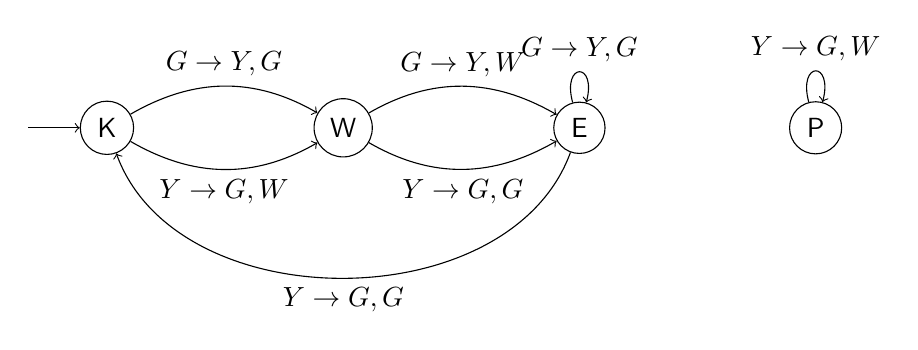
\begin{tikzpicture}
\node[draw, circle] (K) at (0, 0) {\sffamily K};
\node[draw, circle] (W) at (3, 0) {\sffamily W};
\node[draw, circle] (E) at (6, 0) {\sffamily E};
\node[draw, circle] (P) at (9, 0) {\sffamily P};
\draw[->] (-1, 0) to (K);
\draw[->] (K) to[out=-30, in=-150] node[midway, below] {$\q{Y} \rightarrow \q{G}, \q{W}$} (W);
\draw[->] (K) to[out=30, in=150] node[midway, above] {$\q{G} \rightarrow \q{Y}, \q{G}$} (W);
\draw[->] (E) to[out=-110, in=-70] node[midway, below] {$\q{Y} \rightarrow \q{G}, \q{G}$} (K);
\draw[->] (E) to[loop above] node[midway, above] {$\q{G} \rightarrow \q{Y}, \q{G}$} (E);
\draw[->] (W) to[out=-30, in=-150] node[midway, below] {$\q{Y} \rightarrow \q{G}, \q{G}$} (E);
\draw[->] (W) to[out=30, in=150] node[midway, above] {$\q{G} \rightarrow \q{Y}, \q{W}$} (E);
\draw[->] (P) to[loop above] node[midway, above] {$\q{Y} \rightarrow \q{G}, \q{W}$} (P);
\end{tikzpicture}

\noindent and 32 machines equivalent to machine \texttt{A3654D0}:

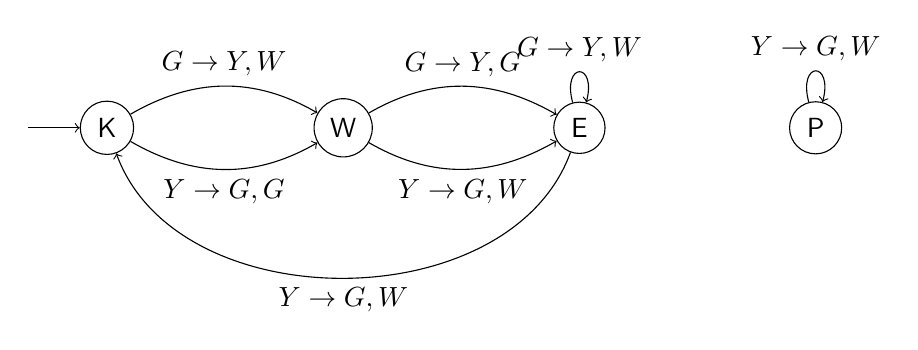
\begin{tikzpicture}
\node[draw, circle] (K) at (0, 0) {\sffamily K};
\node[draw, circle] (W) at (3, 0) {\sffamily W};
\node[draw, circle] (E) at (6, 0) {\sffamily E};
\node[draw, circle] (P) at (9, 0) {\sffamily P};
\draw[->] (-1, 0) to (K);
\draw[->] (K) to[out=-30, in=-150] node[midway, below] {$\q{Y} \rightarrow \q{G}, \q{G}$} (W);
\draw[->] (K) to[out=30, in=150] node[midway, above] {$\q{G} \rightarrow \q{Y}, \q{W}$} (W);
\draw[->] (E) to[out=-110, in=-70] node[midway, below] {$\q{Y} \rightarrow \q{G}, \q{W}$} (K);
\draw[->] (E) to[loop above] node[midway, above] {$\q{G} \rightarrow \q{Y}, \q{W}$} (E);
\draw[->] (W) to[out=-30, in=-150] node[midway, below] {$\q{Y} \rightarrow \q{G}, \q{W}$} (E);
\draw[->] (W) to[out=30, in=150] node[midway, above] {$\q{G} \rightarrow \q{Y}, \q{G}$} (E);
\draw[->] (P) to[loop above] node[midway, above] {$\q{Y} \rightarrow \q{G}, \q{W}$} (P);
\end{tikzpicture}

Tied for third place with 504,454,852 wins and 15,088,237,340 points are 32 machines equivalent to machine \texttt{2DE34F0}:

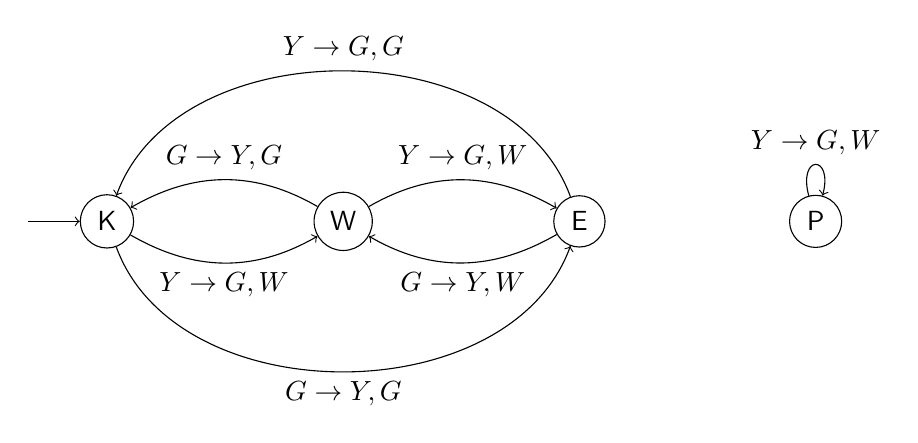
\begin{tikzpicture}
\node[draw, circle] (K) at (0, 0) {\sffamily K};
\node[draw, circle] (W) at (3, 0) {\sffamily W};
\node[draw, circle] (E) at (6, 0) {\sffamily E};
\node[draw, circle] (P) at (9, 0) {\sffamily P};
\draw[->] (-1, 0) to (K);
\draw[->] (K) to[out=-30, in=-150] node[midway, below] {$\q{Y} \rightarrow \q{G}, \q{W}$} (W);
\draw[->] (K) to[out=-70, in=-110] node[midway, below] {$\q{G} \rightarrow \q{Y}, \q{G}$} (E);
\draw[->] (E) to[out=110, in=70] node[midway, above] {$\q{Y} \rightarrow \q{G}, \q{G}$} (K);
\draw[->] (E) to[out=-150, in=-30] node[midway, below] {$\q{G} \rightarrow \q{Y}, \q{W}$} (W);
\draw[->] (W) to[out=30, in=150] node[midway, above] {$\q{Y} \rightarrow \q{G}, \q{W}$} (E);
\draw[->] (W) to[out=150, in=30] node[midway, above] {$\q{G} \rightarrow \q{Y}, \q{G}$} (K);
\draw[->] (P) to[loop above] node[midway, above] {$\q{Y} \rightarrow \q{G}, \q{W}$} (P);
\end{tikzpicture}

\noindent and 32 machines equivalent to machine \texttt{A56BC70}:

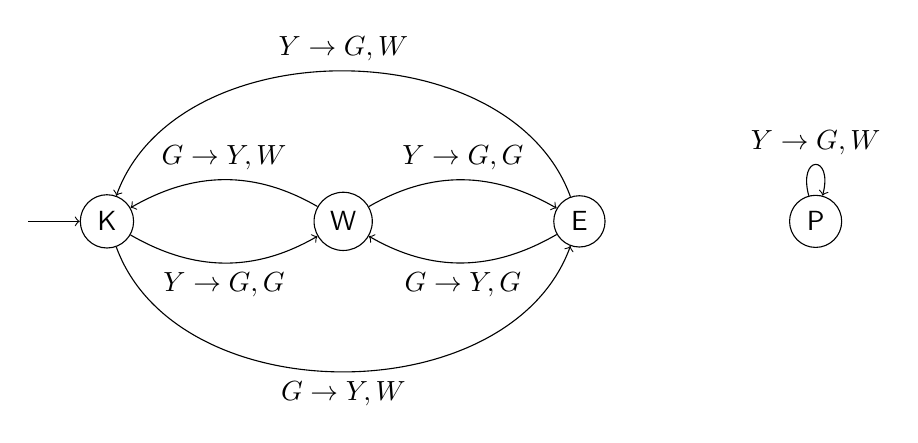
\begin{tikzpicture}
\node[draw, circle] (K) at (0, 0) {\sffamily K};
\node[draw, circle] (W) at (3, 0) {\sffamily W};
\node[draw, circle] (E) at (6, 0) {\sffamily E};
\node[draw, circle] (P) at (9, 0) {\sffamily P};
\draw[->] (-1, 0) to (K);
\draw[->] (K) to[out=-30, in=-150] node[midway, below] {$\q{Y} \rightarrow \q{G}, \q{G}$} (W);
\draw[->] (K) to[out=-70, in=-110] node[midway, below] {$\q{G} \rightarrow \q{Y}, \q{W}$} (E);
\draw[->] (E) to[out=110, in=70] node[midway, above] {$\q{Y} \rightarrow \q{G}, \q{W}$} (K);
\draw[->] (E) to[out=-150, in=-30] node[midway, below] {$\q{G} \rightarrow \q{Y}, \q{G}$} (W);
\draw[->] (W) to[out=30, in=150] node[midway, above] {$\q{Y} \rightarrow \q{G}, \q{G}$} (E);
\draw[->] (W) to[out=150, in=30] node[midway, above] {$\q{G} \rightarrow \q{Y}, \q{W}$} (K);
\draw[->] (P) to[loop above] node[midway, above] {$\q{Y} \rightarrow \q{G}, \q{W}$} (P);
\end{tikzpicture}

Tied for fifth place with 504,388,246 wins and 15,152,181,364 points are 32 machines equivalent to machine \texttt{AB634D0}:

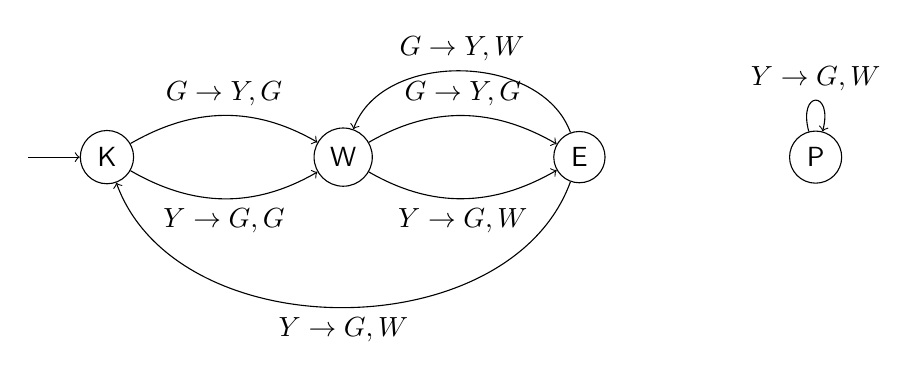
\begin{tikzpicture}
\node[draw, circle] (K) at (0, 0) {\sffamily K};
\node[draw, circle] (W) at (3, 0) {\sffamily W};
\node[draw, circle] (E) at (6, 0) {\sffamily E};
\node[draw, circle] (P) at (9, 0) {\sffamily P};
\draw[->] (-1, 0) to (K);
\draw[->] (K) to[out=-30, in=-150] node[midway, below] {$\q{Y} \rightarrow \q{G}, \q{G}$} (W);
\draw[->] (K) to[out=30, in=150] node[midway, above] {$\q{G} \rightarrow \q{Y}, \q{G}$} (W);
\draw[->] (E) to[out=-110, in=-70] node[midway, below] {$\q{Y} \rightarrow \q{G}, \q{W}$} (K);
\draw[->] (E) to[out=110, in=70] node[midway, above] {$\q{G} \rightarrow \q{Y}, \q{W}$} (W);
\draw[->] (W) to[out=-30, in=-150] node[midway, below] {$\q{Y} \rightarrow \q{G}, \q{W}$} (E);
\draw[->] (W) to[out=30, in=150] node[midway, above] {$\q{G} \rightarrow \q{Y}, \q{G}$} (E);
\draw[->] (P) to[loop above] node[midway, above] {$\q{Y} \rightarrow \q{G}, \q{W}$} (P);
\end{tikzpicture}

\noindent and 32 machines equivalent to machine \texttt{23EBC50}:

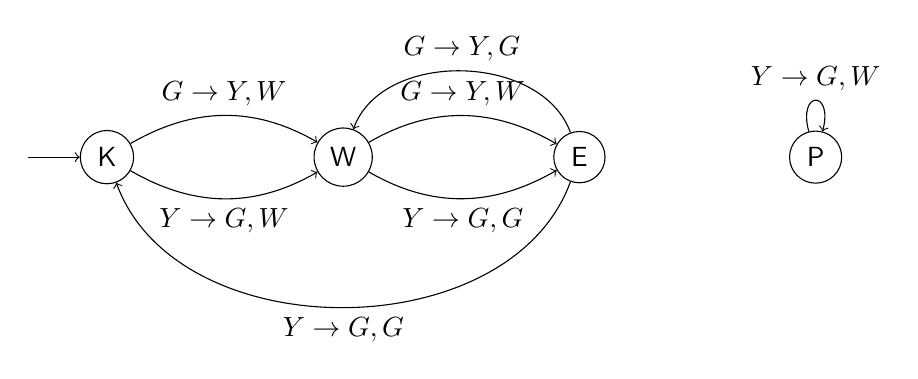
\begin{tikzpicture}
\node[draw, circle] (K) at (0, 0) {\sffamily K};
\node[draw, circle] (W) at (3, 0) {\sffamily W};
\node[draw, circle] (E) at (6, 0) {\sffamily E};
\node[draw, circle] (P) at (9, 0) {\sffamily P};
\draw[->] (-1, 0) to (K);
\draw[->] (K) to[out=-30, in=-150] node[midway, below] {$\q{Y} \rightarrow \q{G}, \q{W}$} (W);
\draw[->] (K) to[out=30, in=150] node[midway, above] {$\q{G} \rightarrow \q{Y}, \q{W}$} (W);
\draw[->] (E) to[out=-110, in=-70] node[midway, below] {$\q{Y} \rightarrow \q{G}, \q{G}$} (K);
\draw[->] (E) to[out=110, in=70] node[midway, above] {$\q{G} \rightarrow \q{Y}, \q{G}$} (W);
\draw[->] (W) to[out=-30, in=-150] node[midway, below] {$\q{Y} \rightarrow \q{G}, \q{G}$} (E);
\draw[->] (W) to[out=30, in=150] node[midway, above] {$\q{G} \rightarrow \q{Y}, \q{W}$} (E);
\draw[->] (P) to[loop above] node[midway, above] {$\q{Y} \rightarrow \q{G}, \q{W}$} (P);
\end{tikzpicture}

Tied for seventh place with 504,120,538 wins and 15,272,577,672 points are 32 machines equivalent to machine \texttt{23C74D0}:

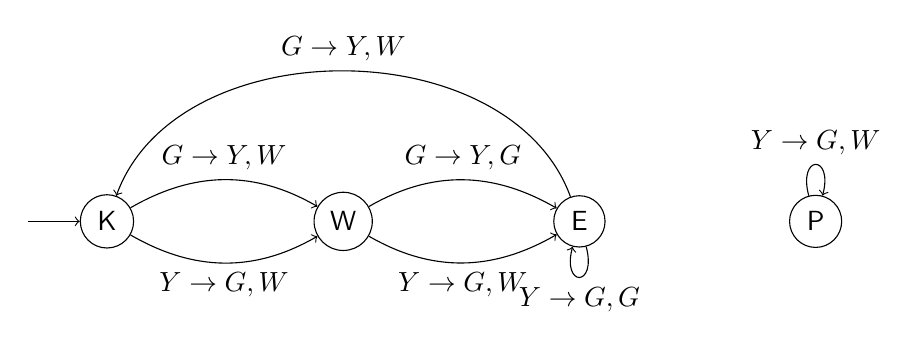
\begin{tikzpicture}
\node[draw, circle] (K) at (0, 0) {\sffamily K};
\node[draw, circle] (W) at (3, 0) {\sffamily W};
\node[draw, circle] (E) at (6, 0) {\sffamily E};
\node[draw, circle] (P) at (9, 0) {\sffamily P};
\draw[->] (-1, 0) to (K);
\draw[->] (K) to[out=-30, in=-150] node[midway, below] {$\q{Y} \rightarrow \q{G}, \q{W}$} (W);
\draw[->] (K) to[out=30, in=150] node[midway, above] {$\q{G} \rightarrow \q{Y}, \q{W}$} (W);
\draw[->] (E) to[loop below] node[midway, below] {$\q{Y} \rightarrow \q{G}, \q{G}$} (E);
\draw[->] (E) to[out=110, in=70] node[midway, above] {$\q{G} \rightarrow \q{Y}, \q{W}$} (K);
\draw[->] (W) to[out=-30, in=-150] node[midway, below] {$\q{Y} \rightarrow \q{G}, \q{W}$} (E);
\draw[->] (W) to[out=30, in=150] node[midway, above] {$\q{G} \rightarrow \q{Y}, \q{G}$} (E);
\draw[->] (P) to[loop above] node[midway, above] {$\q{Y} \rightarrow \q{G}, \q{W}$} (P);
\end{tikzpicture}

\noindent and 32 machines equivalent to machine \texttt{AB4FC50}:

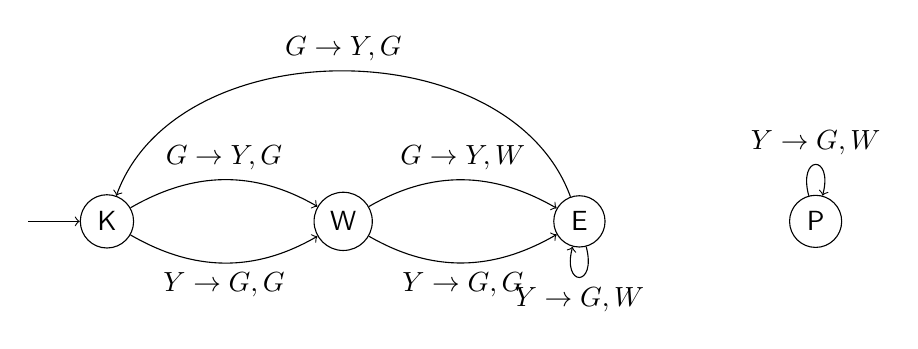
\begin{tikzpicture}
\node[draw, circle] (K) at (0, 0) {\sffamily K};
\node[draw, circle] (W) at (3, 0) {\sffamily W};
\node[draw, circle] (E) at (6, 0) {\sffamily E};
\node[draw, circle] (P) at (9, 0) {\sffamily P};
\draw[->] (-1, 0) to (K);
\draw[->] (K) to[out=-30, in=-150] node[midway, below] {$\q{Y} \rightarrow \q{G}, \q{G}$} (W);
\draw[->] (K) to[out=30, in=150] node[midway, above] {$\q{G} \rightarrow \q{Y}, \q{G}$} (W);
\draw[->] (E) to[loop below] node[midway, below] {$\q{Y} \rightarrow \q{G}, \q{W}$} (E);
\draw[->] (E) to[out=110, in=70] node[midway, above] {$\q{G} \rightarrow \q{Y}, \q{G}$} (K);
\draw[->] (W) to[out=-30, in=-150] node[midway, below] {$\q{Y} \rightarrow \q{G}, \q{G}$} (E);
\draw[->] (W) to[out=30, in=150] node[midway, above] {$\q{G} \rightarrow \q{Y}, \q{W}$} (E);
\draw[->] (P) to[loop above] node[midway, above] {$\q{Y} \rightarrow \q{G}, \q{W}$} (P);
\end{tikzpicture}

Tied for ninth place with 504,115,038 wins and 14,981,424,366 points are 32 machines equivalent to machine \texttt{2DE34B0}:

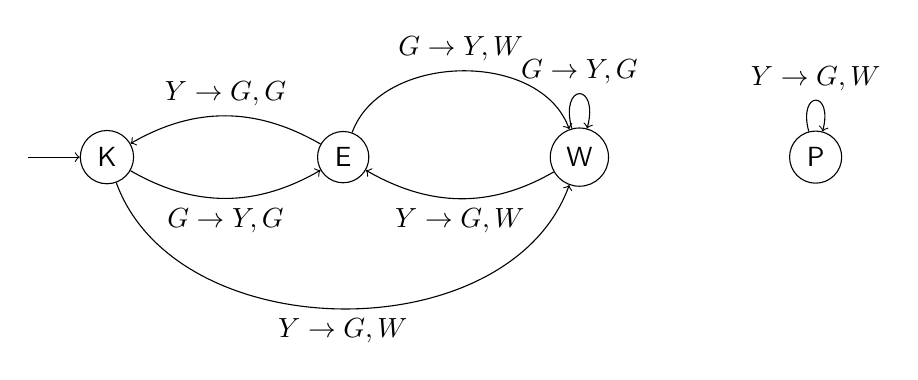
\begin{tikzpicture}
\node[draw, circle] (K) at (0, 0) {\sffamily K};
\node[draw, circle] (E) at (3, 0) {\sffamily E};
\node[draw, circle] (W) at (6, 0) {\sffamily W};
\node[draw, circle] (P) at (9, 0) {\sffamily P};
\draw[->] (-1, 0) to (K);
\draw[->] (K) to[out=-70, in=-110] node[midway, below] {$\q{Y} \rightarrow \q{G}, \q{W}$} (W);
\draw[->] (K) to[out=-30, in=-150] node[midway, below] {$\q{G} \rightarrow \q{Y}, \q{G}$} (E);
\draw[->] (E) to[out=150, in=30] node[midway, above] {$\q{Y} \rightarrow \q{G}, \q{G}$} (K);
\draw[->] (E) to[out=70, in=110] node[midway, above] {$\q{G} \rightarrow \q{Y}, \q{W}$} (W);
\draw[->] (W) to[out=-150, in=-30] node[midway, below] {$\q{Y} \rightarrow \q{G}, \q{W}$} (E);
\draw[->] (W) to[loop above] node[midway, above] {$\q{G} \rightarrow \q{Y}, \q{G}$} (W);
\draw[->] (P) to[loop above] node[midway, above] {$\q{Y} \rightarrow \q{G}, \q{W}$} (P);
\end{tikzpicture}

\noindent and 32 machines equivalent to machine \texttt{A56BC30}:

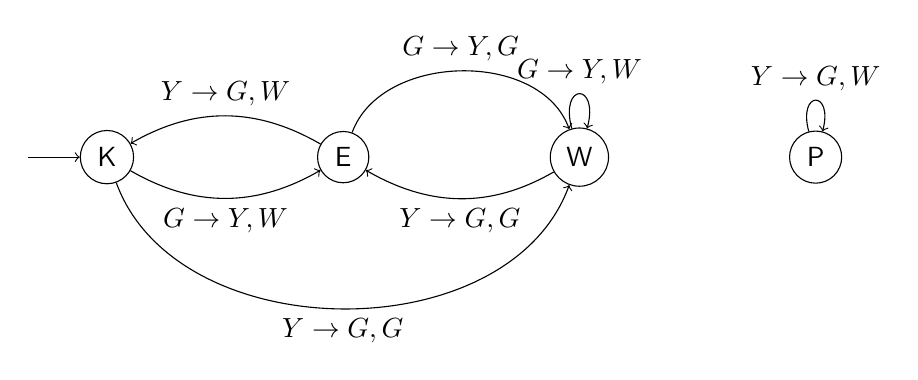
\begin{tikzpicture}
\node[draw, circle] (K) at (0, 0) {\sffamily K};
\node[draw, circle] (E) at (3, 0) {\sffamily E};
\node[draw, circle] (W) at (6, 0) {\sffamily W};
\node[draw, circle] (P) at (9, 0) {\sffamily P};
\draw[->] (-1, 0) to (K);
\draw[->] (K) to[out=-70, in=-110] node[midway, below] {$\q{Y} \rightarrow \q{G}, \q{G}$} (W);
\draw[->] (K) to[out=-30, in=-150] node[midway, below] {$\q{G} \rightarrow \q{Y}, \q{W}$} (E);
\draw[->] (E) to[out=150, in=30] node[midway, above] {$\q{Y} \rightarrow \q{G}, \q{W}$} (K);
\draw[->] (E) to[out=70, in=110] node[midway, above] {$\q{G} \rightarrow \q{Y}, \q{G}$} (W);
\draw[->] (W) to[out=-150, in=-30] node[midway, below] {$\q{Y} \rightarrow \q{G}, \q{G}$} (E);
\draw[->] (W) to[loop above] node[midway, above] {$\q{G} \rightarrow \q{Y}, \q{W}$} (W);
\draw[->] (P) to[loop above] node[midway, above] {$\q{Y} \rightarrow \q{G}, \q{W}$} (P);
\end{tikzpicture}

All of the transitions of the top ten equivalence sets always earn points
by changing the colour of tiles. None of the equivalence sets ever transition to
the Platypus state. The size of the equivalence sets is due to there being 16
configurations for the transition from Platypus upon reading a Yellow cell,
which is irrelevant as the Platypus state is unreachable, and 2 ways to assign
Emu and Wombat machines due to mirroring.

It is immediately evident that all positions in the top ten are ties between
two equivalence sets with similar structure. The only difference is that the
directions moved for every transition are flipped;
flipping the directions does not produce an equivalent machine, but flipping does
produce a machine which performs identically in a full tournament. A
match between machines $M_1$ and $M_2$ will have the same outcome as a
match between $M_1$ with directions flipped and $M_2$ with directions flipped.

\section{Player 1}

32 equivalence sets tied for first place as the first player, with
260,757,230 wins and 6,768,864,104 points. The equivalence sets include 2
machines equivalent to machine \texttt{3A34D2}:

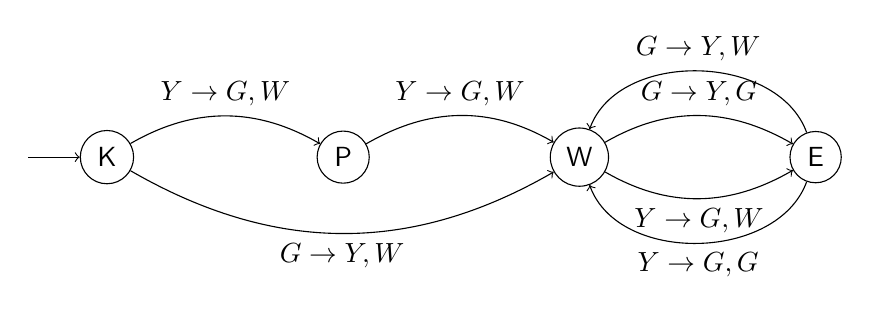
\begin{tikzpicture}
\node[draw, circle] (K) at (0, 0) {\sffamily K};
\node[draw, circle] (P) at (3, 0) {\sffamily P};
\node[draw, circle] (W) at (6, 0) {\sffamily W};
\node[draw, circle] (E) at (9, 0) {\sffamily E};
\draw[->] (-1, 0) to (K);
\draw[->] (K) to[out=30, in=150] node[midway, above] {$\q{Y} \rightarrow \q{G}, \q{W}$} (P);
\draw[->] (K) to[out=-30, in=-150] node[midway, below] {$\q{G} \rightarrow \q{Y}, \q{W}$} (W);
\draw[->] (E) to[out=-110, in=-70] node[midway, below] {$\q{Y} \rightarrow \q{G}, \q{G}$} (W);
\draw[->] (E) to[out=110, in=70] node[midway, above] {$\q{G} \rightarrow \q{Y}, \q{W}$} (W);
\draw[->] (W) to[out=-30, in=-150] node[midway, below] {$\q{Y} \rightarrow \q{G}, \q{W}$} (E);
\draw[->] (W) to[out=30, in=150] node[midway, above] {$\q{G} \rightarrow \q{Y}, \q{G}$} (E);
\draw[->] (P) to[out=30, in=150] node[midway, above] {$\q{Y} \rightarrow \q{G}, \q{W}$} (W);
\end{tikzpicture}

\noindent 2 machines equivalent to machine \texttt{8F2BC5A}:

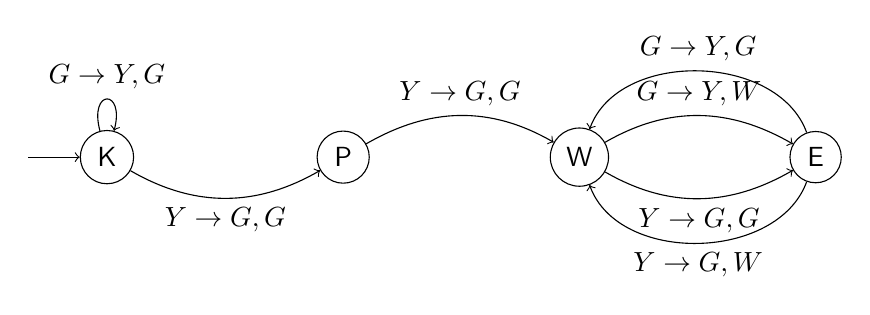
\begin{tikzpicture}
\node[draw, circle] (K) at (0, 0) {\sffamily K};
\node[draw, circle] (P) at (3, 0) {\sffamily P};
\node[draw, circle] (W) at (6, 0) {\sffamily W};
\node[draw, circle] (E) at (9, 0) {\sffamily E};
\draw[->] (-1, 0) to (K);
\draw[->] (K) to[out=-30, in=-150] node[midway, below] {$\q{Y} \rightarrow \q{G}, \q{G}$} (P);
\draw[->] (K) to[loop above] node[midway, above] {$\q{G} \rightarrow \q{Y}, \q{G}$} (K);
\draw[->] (E) to[out=-110, in=-70] node[midway, below] {$\q{Y} \rightarrow \q{G}, \q{W}$} (W);
\draw[->] (E) to[out=110, in=70] node[midway, above] {$\q{G} \rightarrow \q{Y}, \q{G}$} (W);
\draw[->] (W) to[out=-30, in=-150] node[midway, below] {$\q{Y} \rightarrow \q{G}, \q{G}$} (E);
\draw[->] (W) to[out=30, in=150] node[midway, above] {$\q{G} \rightarrow \q{Y}, \q{W}$} (E);
\draw[->] (P) to[out=30, in=150] node[midway, above] {$\q{Y} \rightarrow \q{G}, \q{G}$} (W);
\end{tikzpicture}

\noindent 2 machines equivalent to machine \texttt{05A34D2}:

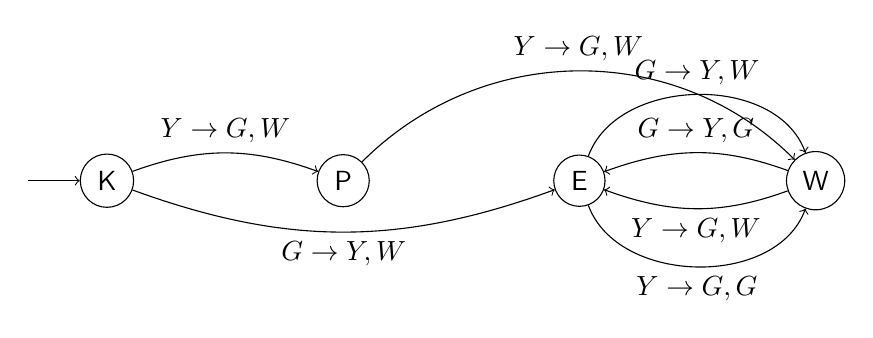
\begin{tikzpicture}
\node[draw, circle] (K) at (0, 0) {\sffamily K};
\node[draw, circle] (P) at (3, 0) {\sffamily P};
\node[draw, circle] (E) at (6, 0) {\sffamily E};
\node[draw, circle] (W) at (9, 0) {\sffamily W};
\draw[->] (-1, 0) to (K);
\draw[->] (K) to[out=-20, in=-160] node[midway, below] {$\q{G} \rightarrow \q{Y}, \q{W}$} (E);
\draw[->] (P) to[out=45, in=135] node[midway, above] {$\q{Y} \rightarrow \q{G}, \q{W}$} (W);
\draw[->] (K) to[out=20, in=160] node[midway, above] {$\q{Y} \rightarrow \q{G}, \q{W}$} (P);
\draw[->] (E) to[out=-70, in=-110] node[midway, below] {$\q{Y} \rightarrow \q{G}, \q{G}$} (W);
\draw[->] (E) to[out=70, in=110] node[midway, above] {$\q{G} \rightarrow \q{Y}, \q{W}$} (W);
\draw[->] (W) to[out=-160, in=-20] node[midway, below] {$\q{Y} \rightarrow \q{G}, \q{W}$} (E);
\draw[->] (W) to[out=160, in=20] node[midway, above] {$\q{G} \rightarrow \q{Y}, \q{G}$} (E);
\end{tikzpicture}

\noindent 2 machines equivalent to machine \texttt{822BC5A}:

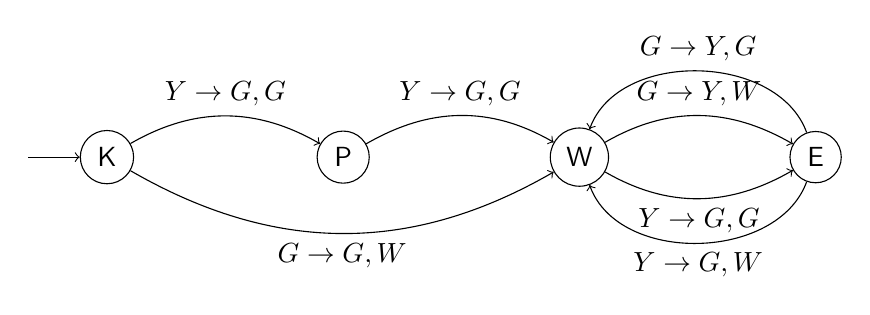
\begin{tikzpicture}
\node[draw, circle] (K) at (0, 0) {\sffamily K};
\node[draw, circle] (P) at (3, 0) {\sffamily P};
\node[draw, circle] (W) at (6, 0) {\sffamily W};
\node[draw, circle] (E) at (9, 0) {\sffamily E};
\draw[->] (-1, 0) to (K);
\draw[->] (K) to[out=30, in=150] node[midway, above] {$\q{Y} \rightarrow \q{G}, \q{G}$} (P);
\draw[->] (K) to[out=-30, in=-150] node[midway, below] {$\q{G} \rightarrow \q{G}, \q{W}$} (W);
\draw[->] (E) to[out=-110, in=-70] node[midway, below] {$\q{Y} \rightarrow \q{G}, \q{W}$} (W);
\draw[->] (E) to[out=110, in=70] node[midway, above] {$\q{G} \rightarrow \q{Y}, \q{G}$} (W);
\draw[->] (W) to[out=-30, in=-150] node[midway, below] {$\q{Y} \rightarrow \q{G}, \q{G}$} (E);
\draw[->] (W) to[out=30, in=150] node[midway, above] {$\q{G} \rightarrow \q{Y}, \q{W}$} (E);
\draw[->] (P) to[out=30, in=150] node[midway, above] {$\q{Y} \rightarrow \q{G}, \q{G}$} (W);
\end{tikzpicture}

\noindent and 2 machines equivalent to machine \texttt{0CA34D2}:

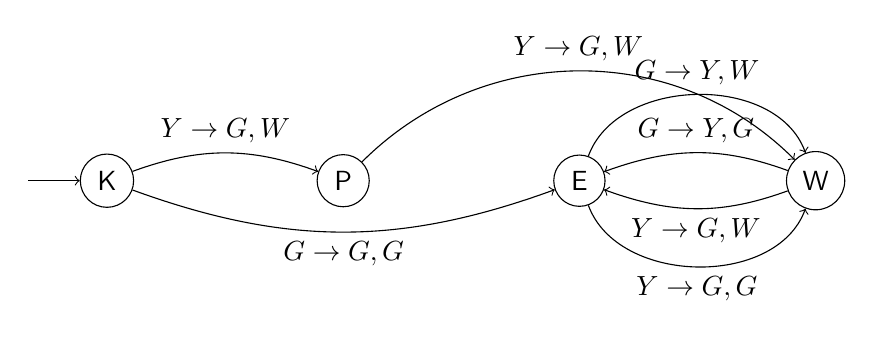
\begin{tikzpicture}
\node[draw, circle] (K) at (0, 0) {\sffamily K};
\node[draw, circle] (P) at (3, 0) {\sffamily P};
\node[draw, circle] (E) at (6, 0) {\sffamily E};
\node[draw, circle] (W) at (9, 0) {\sffamily W};
\draw[->] (-1, 0) to (K);
\draw[->] (K) to[out=-20, in=-160] node[midway, below] {$\q{G} \rightarrow \q{G}, \q{G}$} (E);
\draw[->] (P) to[out=45, in=135] node[midway, above] {$\q{Y} \rightarrow \q{G}, \q{W}$} (W);
\draw[->] (K) to[out=20, in=160] node[midway, above] {$\q{Y} \rightarrow \q{G}, \q{W}$} (P);
\draw[->] (E) to[out=-70, in=-110] node[midway, below] {$\q{Y} \rightarrow \q{G}, \q{G}$} (W);
\draw[->] (E) to[out=70, in=110] node[midway, above] {$\q{G} \rightarrow \q{Y}, \q{W}$} (W);
\draw[->] (W) to[out=-160, in=-20] node[midway, below] {$\q{Y} \rightarrow \q{G}, \q{W}$} (E);
\draw[->] (W) to[out=160, in=20] node[midway, above] {$\q{G} \rightarrow \q{Y}, \q{G}$} (E);
\end{tikzpicture}

Half of the redundancy can be explained by the forementioned flipping of directions,
leaving a 16-way tie. The only remaining difference between the machines is the
transition from the Kangaroo state upon reading a Green cell, which has 16 possible
configurations. The transition is never used as the first player always
reads yellow in its first turn, and none of the machines can reach the
Kangaroo state again. The Platypus state is however live in all of the top 32 equivalence
sets, but it also does not seem like the machines will halt the game because
a machine can only be in the Platypus state in its second turn, and there were not
enough turns before for the cell under the machine to be Green.

\section{Player 2}

Tied for first place with 244,410,400 wins and 8,048,411,604 points are 32 machines equivalent to machine \texttt{A56BC30}:

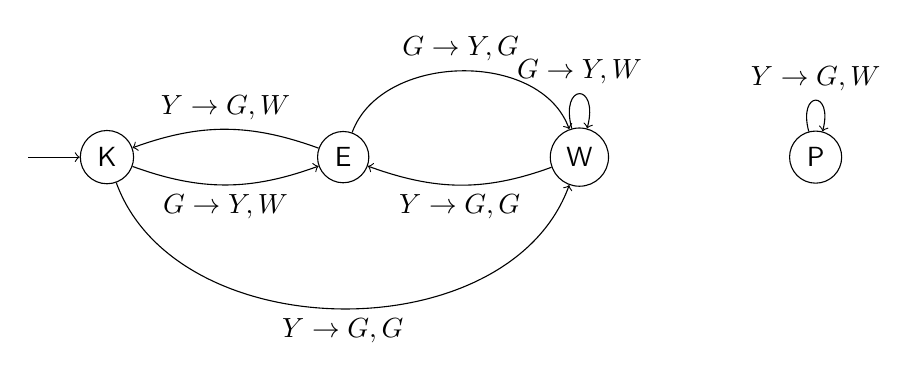
\begin{tikzpicture}
\node[draw, circle] (K) at (0, 0) {\sffamily K};
\node[draw, circle] (E) at (3, 0) {\sffamily E};
\node[draw, circle] (W) at (6, 0) {\sffamily W};
\node[draw, circle] (P) at (9, 0) {\sffamily P};
\draw[->] (-1, 0) to (K);
\draw[->] (K) to[out=-70, in=-110] node[midway, below] {$\q{Y} \rightarrow \q{G}, \q{G}$} (W);
\draw[->] (K) to[out=-20, in=-160] node[midway, below] {$\q{G} \rightarrow \q{Y}, \q{W}$} (E);
\draw[->] (E) to[out=160, in=20] node[midway, above] {$\q{Y} \rightarrow \q{G}, \q{W}$} (K);
\draw[->] (E) to[out=70, in=110] node[midway, above] {$\q{G} \rightarrow \q{Y}, \q{G}$} (W);
\draw[->] (W) to[out=-160, in=-20] node[midway, below] {$\q{Y} \rightarrow \q{G}, \q{G}$} (E);
\draw[->] (W) to[loop above] node[midway, above] {$\q{G} \rightarrow \q{Y}, \q{W}$} (W);
\draw[->] (P) to[loop above] node[midway, above] {$\q{Y} \rightarrow \q{G}, \q{W}$} (P);
\end{tikzpicture}

\noindent and 32 machines equivalent to machine \texttt{2DE34B0}:

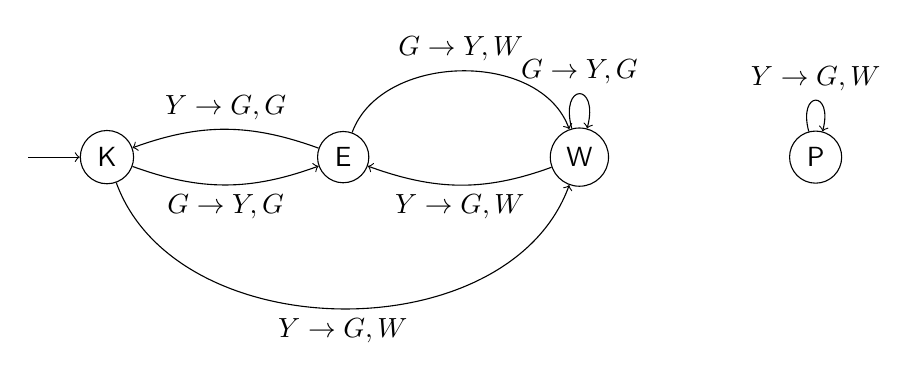
\begin{tikzpicture}
\node[draw, circle] (K) at (0, 0) {\sffamily K};
\node[draw, circle] (E) at (3, 0) {\sffamily E};
\node[draw, circle] (W) at (6, 0) {\sffamily W};
\node[draw, circle] (P) at (9, 0) {\sffamily P};
\draw[->] (-1, 0) to (K);
\draw[->] (K) to[out=-70, in=-110] node[midway, below] {$\q{Y} \rightarrow \q{G}, \q{W}$} (W);
\draw[->] (K) to[out=-20, in=-160] node[midway, below] {$\q{G} \rightarrow \q{Y}, \q{G}$} (E);
\draw[->] (E) to[out=160, in=20] node[midway, above] {$\q{Y} \rightarrow \q{G}, \q{G}$} (K);
\draw[->] (E) to[out=70, in=110] node[midway, above] {$\q{G} \rightarrow \q{Y}, \q{W}$} (W);
\draw[->] (W) to[out=-160, in=-20] node[midway, below] {$\q{Y} \rightarrow \q{G}, \q{W}$} (E);
\draw[->] (W) to[loop above] node[midway, above] {$\q{G} \rightarrow \q{Y}, \q{G}$} (W);
\draw[->] (P) to[loop above] node[midway, above] {$\q{Y} \rightarrow \q{G}, \q{W}$} (P);
\end{tikzpicture}

Tied for third place with 244,295,488 wins and 8,133,793,246 points are 32 machines equivalent to machine \texttt{23EBC50}:

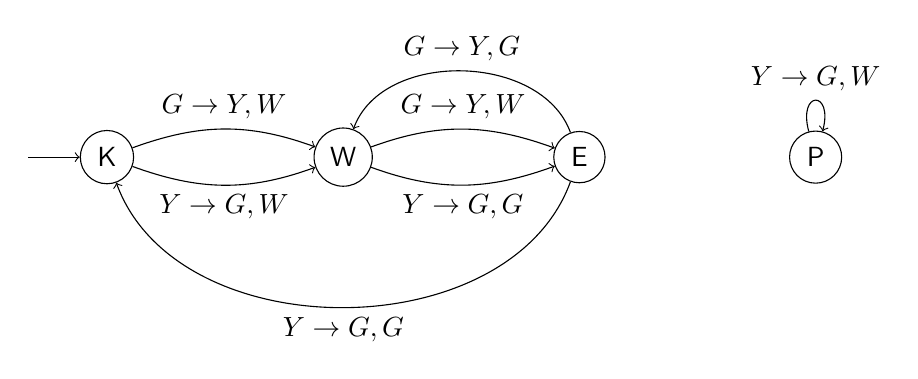
\begin{tikzpicture}
\node[draw, circle] (K) at (0, 0) {\sffamily K};
\node[draw, circle] (W) at (3, 0) {\sffamily W};
\node[draw, circle] (E) at (6, 0) {\sffamily E};
\node[draw, circle] (P) at (9, 0) {\sffamily P};
\draw[->] (-1, 0) to (K);
\draw[->] (E) to[out=-110, in=-70] node[midway, below] {$\q{Y} \rightarrow \q{G}, \q{G}$} (K);
\draw[->] (K) to[out=-20, in=-160] node[midway, below] {$\q{Y} \rightarrow \q{G}, \q{W}$} (W);
\draw[->] (K) to[out=20, in=160] node[midway, above] {$\q{G} \rightarrow \q{Y}, \q{W}$} (W);
\draw[->] (E) to[out=110, in=70] node[midway, above] {$\q{G} \rightarrow \q{Y}, \q{G}$} (W);
\draw[->] (W) to[out=-20, in=-160] node[midway, below] {$\q{Y} \rightarrow \q{G}, \q{G}$} (E);
\draw[->] (W) to[out=20, in=160] node[midway, above] {$\q{G} \rightarrow \q{Y}, \q{W}$} (E);
\draw[->] (P) to[loop above] node[midway, above] {$\q{Y} \rightarrow \q{G}, \q{W}$} (P);
\end{tikzpicture}

\noindent and 32 machines equivalent to machine \texttt{AB634D0}:

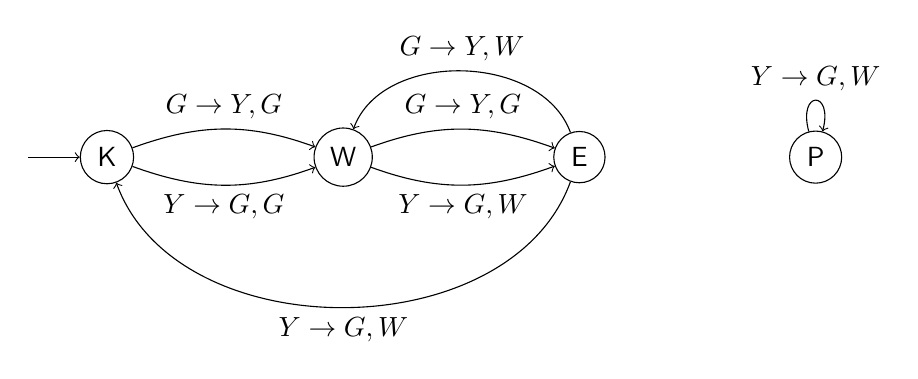
\begin{tikzpicture}
\node[draw, circle] (K) at (0, 0) {\sffamily K};
\node[draw, circle] (W) at (3, 0) {\sffamily W};
\node[draw, circle] (E) at (6, 0) {\sffamily E};
\node[draw, circle] (P) at (9, 0) {\sffamily P};
\draw[->] (-1, 0) to (K);
\draw[->] (E) to[out=-110, in=-70] node[midway, below] {$\q{Y} \rightarrow \q{G}, \q{W}$} (K);
\draw[->] (K) to[out=-20, in=-160] node[midway, below] {$\q{Y} \rightarrow \q{G}, \q{G}$} (W);
\draw[->] (K) to[out=20, in=160] node[midway, above] {$\q{G} \rightarrow \q{Y}, \q{G}$} (W);
\draw[->] (E) to[out=110, in=70] node[midway, above] {$\q{G} \rightarrow \q{Y}, \q{W}$} (W);
\draw[->] (W) to[out=-20, in=-160] node[midway, below] {$\q{Y} \rightarrow \q{G}, \q{W}$} (E);
\draw[->] (W) to[out=20, in=160] node[midway, above] {$\q{G} \rightarrow \q{Y}, \q{G}$} (E);
\draw[->] (P) to[loop above] node[midway, above] {$\q{Y} \rightarrow \q{G}, \q{W}$} (P);
\end{tikzpicture}

In fifth place with 244,268,960 wins and 8,240,095,104 points, 32 machines equivalent to machine \texttt{2BEDE50}:

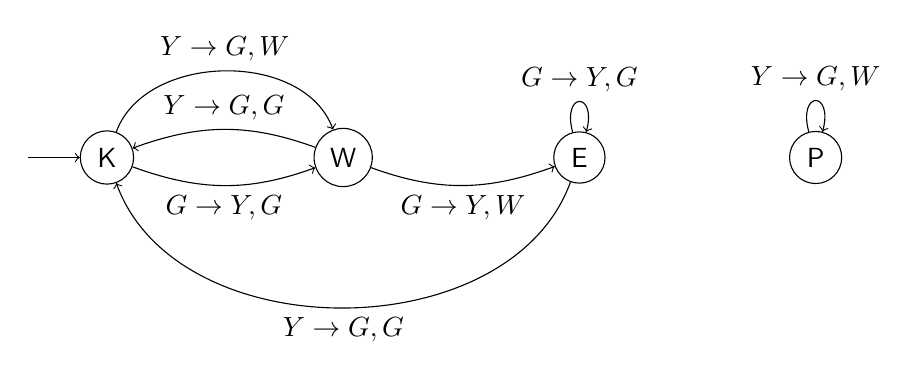
\begin{tikzpicture}
\node[draw, circle] (K) at (0, 0) {\sffamily K};
\node[draw, circle] (W) at (3, 0) {\sffamily W};
\node[draw, circle] (E) at (6, 0) {\sffamily E};
\node[draw, circle] (P) at (9, 0) {\sffamily P};
\draw[->] (-1, 0) to (K);
\draw[->] (E) to[out=-110, in=-70] node[midway, below] {$\q{Y} \rightarrow \q{G}, \q{G}$} (K);
\draw[->] (K) to[out=70, in=110] node[midway, above] {$\q{Y} \rightarrow \q{G}, \q{W}$} (W);
\draw[->] (K) to[out=-20, in=-160] node[midway, below] {$\q{G} \rightarrow \q{Y}, \q{G}$} (W);
\draw[->] (W) to[out=160, in=20] node[midway, above] {$\q{Y} \rightarrow \q{G}, \q{G}$} (K);
\draw[->] (W) to[out=-20, in=-160] node[midway, below] {$\q{G} \rightarrow \q{Y}, \q{W}$} (E);
\draw[->] (E) to[loop above] node[midway, above] {$\q{G} \rightarrow \q{Y}, \q{G}$} (E);
\draw[->] (P) to[loop above] node[midway, above] {$\q{Y} \rightarrow \q{G}, \q{W}$} (P);
\end{tikzpicture}

Only the same sources of redundancy in the full results appear in the
top five equivalence sets for Player 2. Player 1 appears to have an advantage
in the Platypus game as the best machine for Player 1 earns more wins than
the best machine for Player 2, but the best machine for Player 2 earns
more points. This may be due to the Platypus state being dead in all top 5
equivalence sets, so the machines will never attempt to halt the game.